% Author :  Lionel du Peloux
% Contact : lionel.dupeloux@gmail
% Year : 2017

% ===========================
% COMPILER DIRECTIVES
% ===========================
% !TEX encoding = UTF-8 Unicode
% !TEX TS-program = XeLaTeX-shellescape
% !BIB TS-program = biber
% !BIB program = biber

\thispagestyle{empty}
\AddToShipoutPictureBG*{%
	\begin{tikzpicture}[remember picture, overlay, inner sep=0pt]
		\begin{scope}
			\setlength{\pgflinewidth}{0pt}
			\clip (PPbl) rectangle (PPtr);
			\node[anchor=north east] at (PPtr){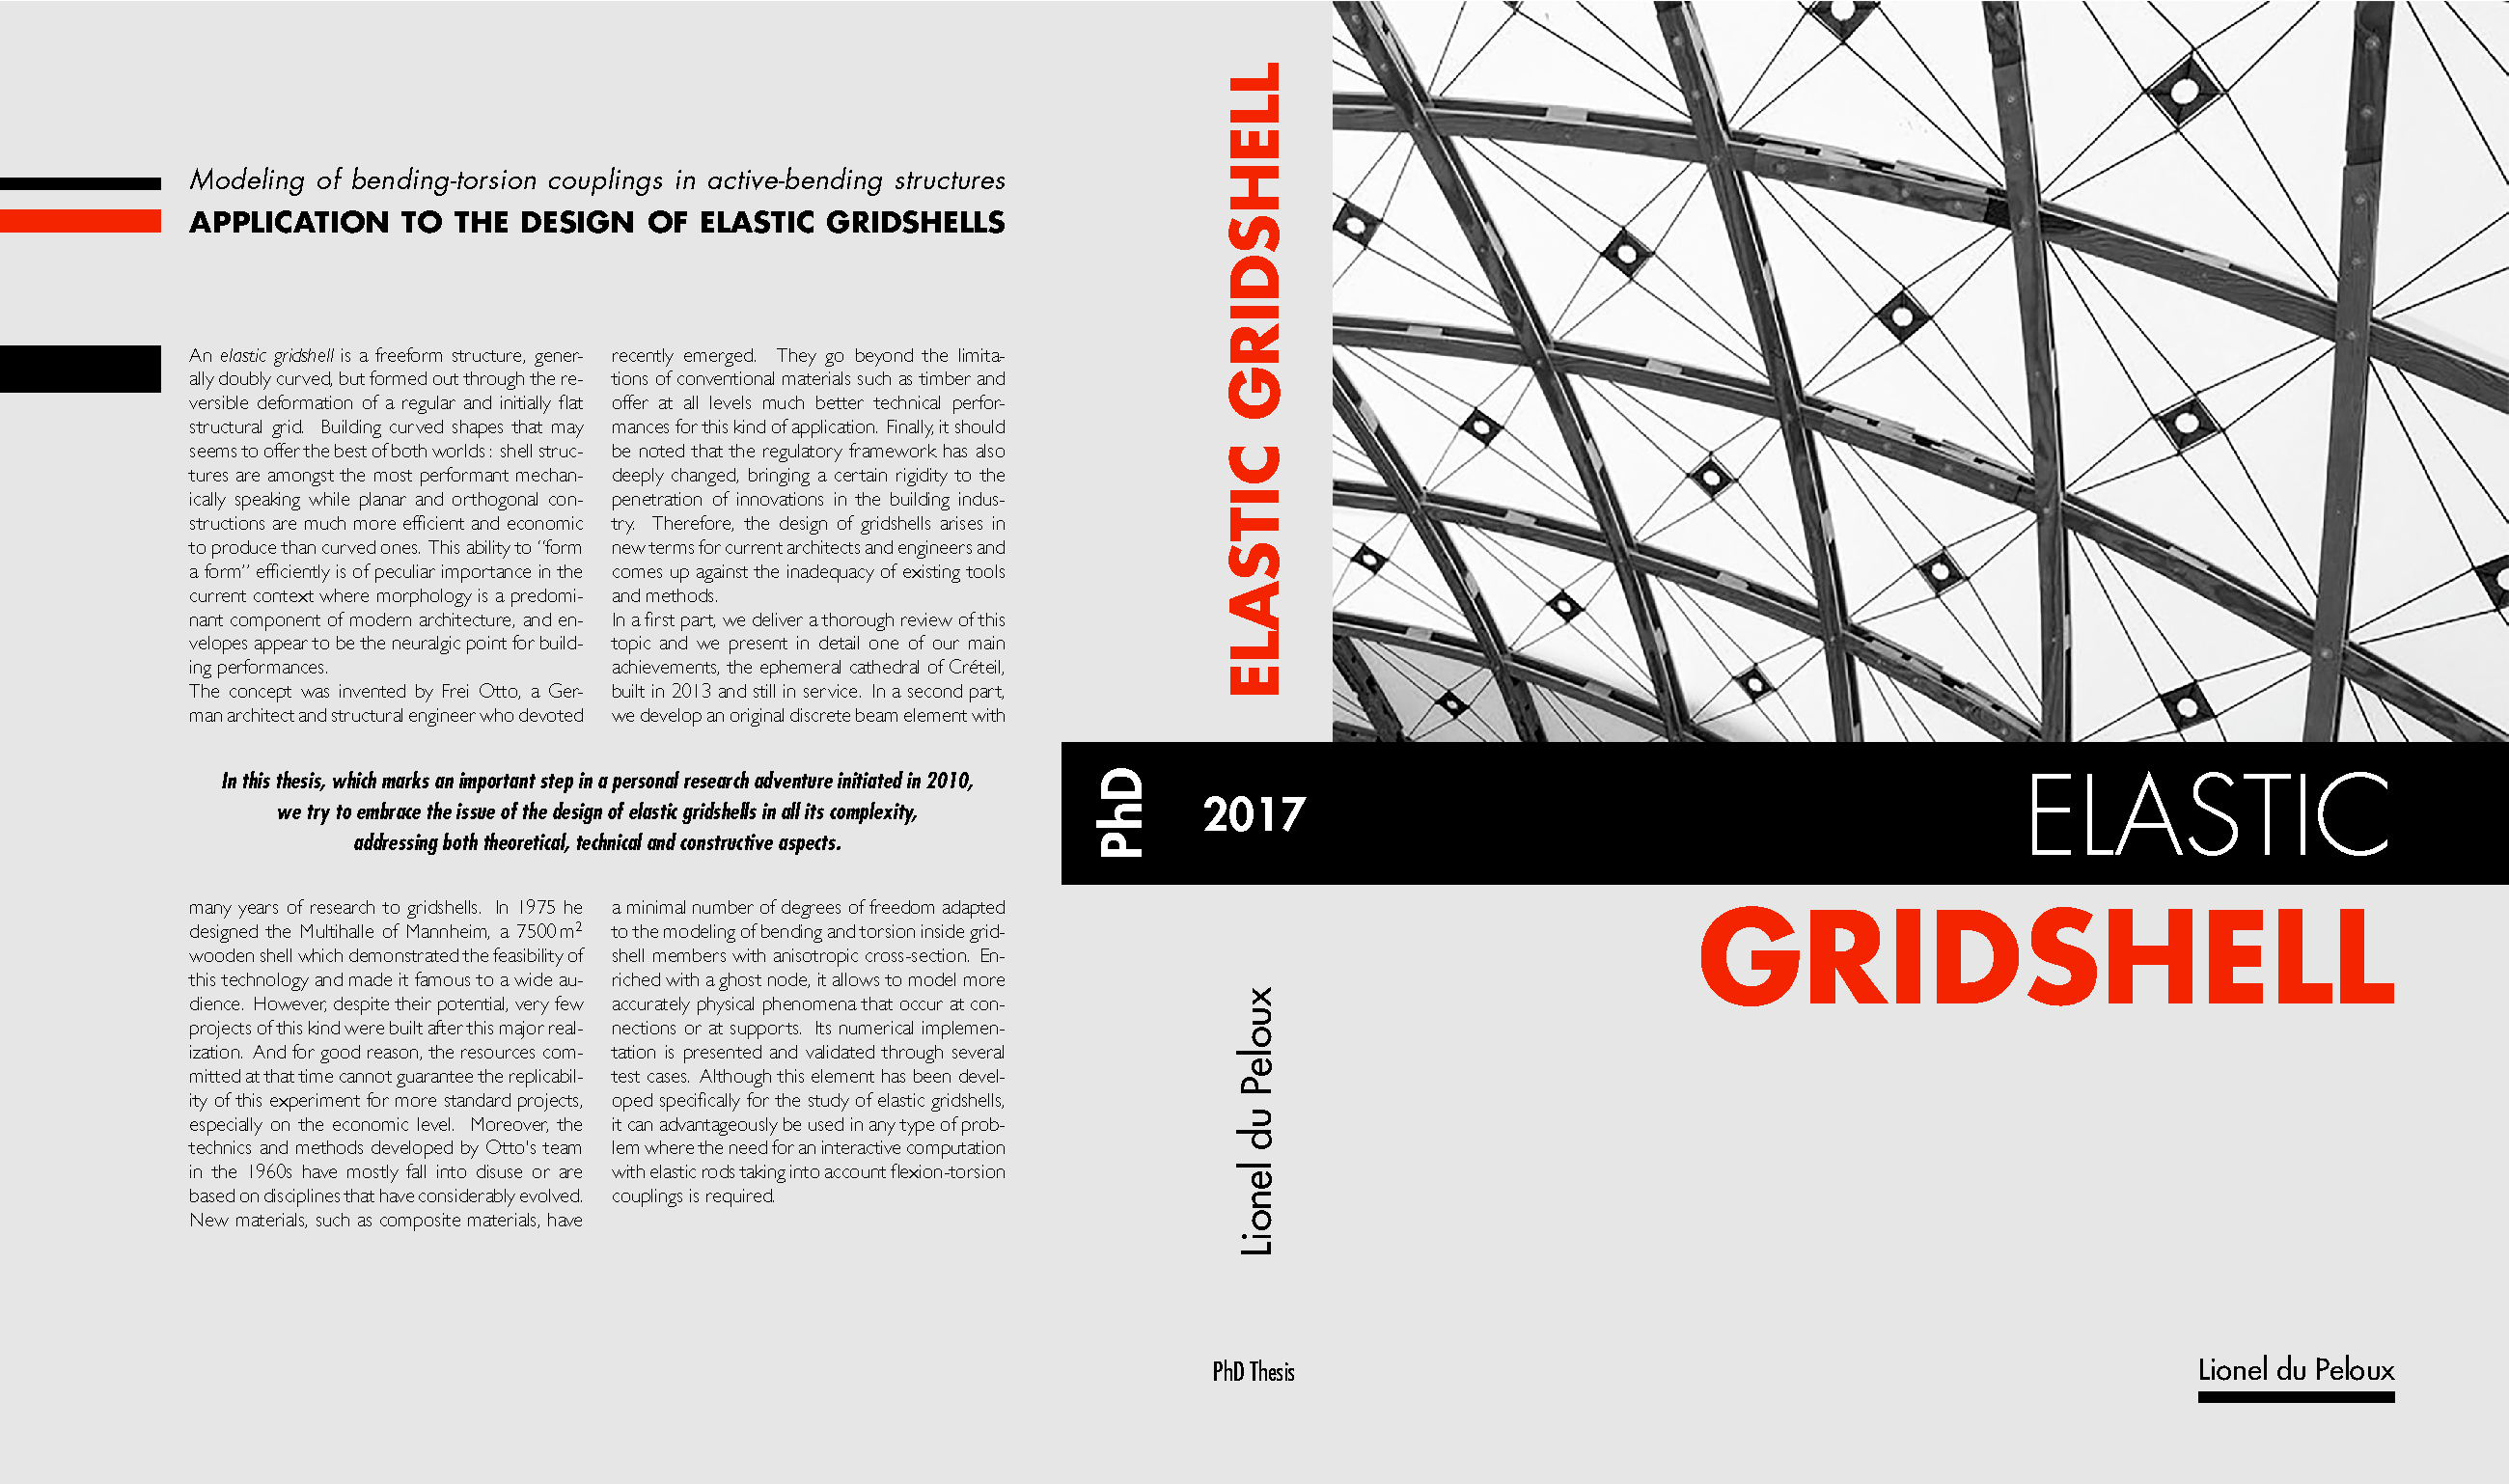
\includegraphics{softcoverwithbleed.pdf}};
		\end{scope}		
	\end{tikzpicture}
}
\hbox{}

\clearpage\hbox{}\thispagestyle{empty}
\clearpage\hbox{}\thispagestyle{empty}

% FONT FAMILY
\newfontfamily\FTRegular{FuturaLT}[Scale = MatchUppercase]
\newfontfamily\FTLight{FuturaLT-Light}[Scale = MatchUppercase]
\newfontfamily\FTBold{FuturaLT-Bold}[Scale = MatchUppercase]
\newfontfamily\FTHeavy{FuturaLT-Heavy}[Scale = MatchUppercase]
\newfontfamily\FTBookOblique{FuturaLT-BookOblique}[Scale = MatchUppercase]
\newfontfamily\FTCondensedBoldOblique{FuturaLT-CondensedBoldOblique}[Scale = MatchUppercase]
\newfontfamily\GSLight{GillSans-Light}[Scale = MatchUppercase]
\newfontfamily\FTCondensed{FuturaLT-Condensed}[Scale = MatchUppercase]

% TYPE FACE BACK COVER
\DeclareRobustCommand{\tfHA}{\FTBookOblique\fontsize{18pt}{22pt}\selectfont}
\DeclareRobustCommand{\tfHC}{\FTLight\fontsize{15pt}{0pt}\selectfont}
\DeclareRobustCommand{\tfHB}{\FTBold\fontsize{24pt}{30pt}\selectfont}
\DeclareRobustCommand{\tfauthor}{\FTLight\fontsize{14pt}{16pt}\selectfont}
\DeclareRobustCommand{\tfquote}{\FTCondensedBoldOblique\large}
\DeclareRobustCommand{\tftxt}{\GSLight\small}
% \sodef\spaceout{}{0pt plus 1fil}{.4em plus 1fil}{0pt}

% \AddToShipoutPictureBG*{%
\begin{tikzpicture}[remember picture, overlay, inner sep=0pt] % ovelay is required, dont now why
	\node[anchor=center] at (PGc){%
		\tfHB
		\fbox{\parbox[c]{0.8\PaperWidth}{%
			\centering
			THE DESIGN OF ELASTIC GRIDSHELLS
	}}};
	\path (PGc) -- (PGt) coordinate[midway] (Pt);
	\node[anchor=center, yshift=0cm] at (Pt){%
		\tfHA%
		\fbox{\parbox[b]{0.8\PaperWidth}{
			\centering
			Modeling of bending-torsion couplings\\ 
			in active-bending structures
	}}};
	\path (PGc) -- (Pt) coordinate[midway] (Pt);
	\node[anchor=center, yshift=0cm] at (Pt){%
		\tfHC%
		\fbox{\parbox[b]{0.8\PaperWidth}{
			\centering
			application to
	}}};
	\node[anchor=south, yshift=1.5cm] at (PGb){%
		\tfauthor%
		\fbox{\parbox[b]{0.8\PaperWidth}{
			\centering
			Lionel du Peloux de Saint Romain\\
			PhD Thesis 2017
	}}};
\end{tikzpicture}
% }

\clearpage\hbox{}\thispagestyle{empty}
\clearpage\hbox{}\thispagestyle{empty}

Thèse soutenue le ...
Jury ...